\documentclass[aspectratio=169, table]{beamer}

\usepackage{listings}
\usepackage{luatexja}

%\usepackage[beamertheme=./praditatheme]{Pradita}

\usetheme{Pradita}

\lstdefinelanguage{bash} {
	keywords={},
	basicstyle=\ttfamily\small,
	keywordstyle=\color{blue}\bfseries,
	ndkeywords={iex},
	ndkeywordstyle=\color{purple}\bfseries,
	sensitive=true,
	commentstyle=\color{gray},
	stringstyle=\color{red},
	numbers=left,
	numberstyle=\tiny\color{gray},
	breaklines=true,
	frame=lines,
	backgroundcolor=\color{lightgray!10},
	tabsize=2,
	comment=[l]{\#},
	morecomment=[s]{/*}{*/},
	commentstyle=\color{gray}\ttfamily,
	stringstyle=\color{purple}\ttfamily,
	showstringspaces=false
}

\lstdefinestyle{JavaStyle}{
language=Java,
basicstyle=\ttfamily\footnotesize,
morekeywords={String, int},
keywordstyle=\color{blue},
commentstyle=\color{gray},
stringstyle=\color{red},
breaklines=true,
showstringspaces=false,
tabsize=2,
captionpos=b,
numbers=left,
numberstyle=\tiny\color{gray},
frame=lines,
backgroundcolor=\color{lightgray!10},
comment=[l]{//},
morecomment=[s]{/*}{*/},
commentstyle=\color{gray}\ttfamily,
string=[s]{'}{'},
morestring=[s]{"}{"},
%	stringstyle=\color{teal}\ttfamily,
%	showstringspaces=false
}

\title{\Huge Microkernel/Plugin\\Architecture\\\vspace{10pt}}
\subtitle{IF231303-Software Architecture}
\author{Alfa Yohannis}
\begin{document}

\frame{\titlepage}

\begin{frame}[fragile]
\frametitle{Contents}
\vspace{10pt}
\begin{columns}[t]
\column{0.5\textwidth}
\tableofcontents[sections={1-4}]

\column{0.5\textwidth}
\tableofcontents[sections={5}]
\end{columns}
\end{frame}

\begin{frame}[fragile]
	\frametitle{Contents}
	\vspace{10pt}
	\begin{columns}[t]
		\column{0.5\textwidth}
		\tableofcontents[sections={6}]
		
		\column{0.5\textwidth}
		\tableofcontents[sections={7}]
	\end{columns}
\end{frame}

\section{Introduction}

\begin{frame}{Introduction}
\begin{columns}
\column{0.5\textwidth}
\begin{itemize}
	\item The need for modular, flexible, and extensible systems is increasing in modern computing.
	\item Software architecture plays a crucial role in determining how systems evolve and adapt to changes.
	\item Two main approaches to achieve modularity and flexibility:
	\begin{itemize}
		\item \textbf{Microkernel}
		\item \textbf{Plugin architecture}
	\end{itemize}
\end{itemize}

\column{0.5\textwidth}
\begin{itemize}
	\item \textbf{Microkernel Architecture:}
	\begin{itemize}
		\item Solution to limitations of monolithic OS with high component dependency.
		\item Only core functions run inside the kernel.
		\item Additional services like file systems, drivers, network placed as user processes.
		\item Benefits: improved security and stability.
	\end{itemize}
\end{itemize}
\end{columns}
\end{frame}

\begin{frame}{Plugin Architecture and Document Overview}
\begin{columns}
\column{0.5\textwidth}
\begin{itemize}
	\item \textbf{Plugin Architecture:}
	\begin{itemize}
		\item Add features dynamically without modifying core code.
		\item Common in IDEs, CMS, multimedia software.
		\item Provides flexibility and ease of expansion.
	\end{itemize}
\end{itemize}

\column{0.5\textwidth}
\begin{itemize}
	\item \textbf{Document Overview:}
	\begin{itemize}
		\item Concepts and implementation:
		\begin{itemize}
			\item Microkernel architecture
			\item Plugin architecture
		\end{itemize}
		\item Covers:
		\begin{itemize}
			\item Historical development
			\item Examples, pros \& cons
			\item Implementation in Java projects
		\end{itemize}
	\end{itemize}
\end{itemize}
\end{columns}
\end{frame}

\section{History and Development}

\begin{frame}{History of Microkernel}
\begin{columns}
\column{0.5\textwidth}
\begin{itemize}
	\item Concept emerged to address monolithic OS limitations.
	\item Monolithic OS:
	\begin{itemize}
		\item All services integrated in one large kernel.
		\item Good performance but low flexibility.
		\item Vulnerable to total system failure.
	\end{itemize}
	\item 1960s-1970s:
	\begin{itemize}
		\item Modular system design research began.
		\item \textbf{THE Operating System} by Edsger Dijkstra (1968).
	\end{itemize}
\end{itemize}

\column{0.5\textwidth}
\begin{itemize}
	\item 1980s:
	\begin{itemize}
		\item \textbf{Mach} at Carnegie Mellon University.
		\item Core functions in kernel (memory, scheduling, IPC).
		\item Other services in user processes.
	\end{itemize}
	\item Performance challenges due to IPC overhead.
	\item 1990s:
	\begin{itemize}
		\item \textbf{L4} microkernel introduced.
		\item Basis for modern systems like QNX and Minix.
	\end{itemize}
\end{itemize}
\end{columns}
\end{frame}

\begin{frame}{History \& Development of Plugin Architecture}
\begin{columns}
\column{0.5\textwidth}
\begin{itemize}
	\item Initially, software built monolithic.
	\item Maintenance and updates became difficult.
	\item 1990s:
	\begin{itemize}
		\item \textbf{Netscape Navigator} and \textbf{Internet Explorer} adopted plugins.
		\item Third-party developers could add features without changing core code.
	\end{itemize}
\end{itemize}

\column{0.5\textwidth}
\begin{itemize}
	\item Plugin concept expanded to:
	\begin{itemize}
		\item Content Management Systems (CMS)
		\item IDEs like Eclipse, Visual Studio
		\item Game platforms like Unreal Engine
	\end{itemize}
	\item Used to improve modularity and flexibility in modern software.
\end{itemize}
\end{columns}
\end{frame}

\begin{frame}{Current Usage}
\begin{columns}
\column{0.5\textwidth}
\begin{itemize}
	\item \textbf{Microkernel Architecture:}
	\begin{itemize}
		\item Real-time operating systems
		\item Embedded systems
		\item Virtualisation hypervisors
	\end{itemize}
\end{itemize}

\column{0.5\textwidth}
\begin{itemize}
	\item \textbf{Plugin Architecture:}
	\begin{itemize}
		\item Large-scale applications
		\item Systems requiring high flexibility and strong modularity
	\end{itemize}
\end{itemize}
\end{columns}
\end{frame}

\section{Real-World Applications}

\begin{frame}{Microkernel and Plugin in Real-World Applications}
\begin{columns}
\column{0.5\textwidth}
\begin{itemize}
	\item Microkernel and Plugin architectures are widely applied in:
	\begin{itemize}
		\item Operating systems
		\item Software applications
		\item Embedded systems
	\end{itemize}
	\item Advantages:
	\begin{itemize}
		\item Modular design
		\item Flexibility
		\item Security
		\item Stability
	\end{itemize}
\end{itemize}
\column{0.5\textwidth}
\begin{itemize}
	\item Manage complex systems effectively.
	\item Ensures better fault isolation and scalability.
	\item Enables developers to extend and adapt systems without affecting core components.
\end{itemize}
\end{columns}
\end{frame}

\subsection{Microkernel Applications in Operating Systems}

\begin{frame}{\Large{Microkernel Applications in Operating Systems}}
\vspace{20pt}
\begin{columns}
\column{0.5\textwidth}
\begin{itemize}
	\item \textbf{QNX:}
	\begin{itemize}
		\item Real-time OS based on microkernel.
		\item Used in automotive, telecom, embedded systems.
		\item System continues running even if components fail.
		\item Applied in vehicle infotainment \& control systems.
	\end{itemize}
	\vspace{0.3cm}
	\item \textbf{MINIX 3:}
	\begin{itemize}
		\item High-reliability microkernel OS.
		\item Kernel components can be updated without shutdown.
		\item Used in Intel Management Engine (Intel ME).
	\end{itemize}
\end{itemize}

\column{0.5\textwidth}
\begin{itemize}
	\item \textbf{L4 Microkernel:}
	\begin{itemize}
		\item Modern microkernel used in:
		\begin{itemize}
			\item Mobile security: \textbf{Qualcomm TrustZone}
			\item Hypervisors in cloud computing
		\end{itemize}
		\item Provides strong isolation and efficiency.
	\end{itemize}
	\vspace{0.3cm}
	\item \textbf{Google Fuchsia:}
	\begin{itemize}
		\item Experimental OS by Google.
		\item Based on Zircon microkernel.
		\item Designed to be modular and adaptable.
		\item Supports smartphones to embedded systems.
	\end{itemize}
\end{itemize}
\end{columns}
\end{frame}


\subsection{Plugin Architecture Applications in Software}

\begin{frame}{Plugin Applications: IDEs and CMS}
\begin{columns}
\column{0.5\textwidth}
\begin{itemize}
	\item \textbf{IDEs:}
	\begin{itemize}
		\item Examples:
		\begin{itemize}
			\item \textbf{Eclipse}, \textbf{Visual Studio}, \textbf{IntelliJ IDEA}
		\end{itemize}
		\item Plugins add:
		\begin{itemize}
			\item Language support
			\item Debugging tools
			\item Git integration
		\end{itemize}
	\end{itemize}
\end{itemize}
\column{0.5\textwidth}
\begin{itemize}
	\item \textbf{CMS:}
	\begin{itemize}
		\item Examples:
		\begin{itemize}
			\item \textbf{WordPress}, \textbf{Drupal}, \textbf{Joomla}
		\end{itemize}
		\item Plugins provide:
		\begin{itemize}
			\item SEO optimisation
			\item E-commerce features
			\item Contact forms
			\item Social media integration
		\end{itemize}
	\end{itemize}
\end{itemize}
\end{columns}
\end{frame}

\begin{frame}{\Large{Plugin Applications: Browsers, Multimedia, and Game Engines}}

\begin{columns}
\column{0.5\textwidth}
\begin{itemize}
	\item \textbf{Web Browsers:}
	\begin{itemize}
		\item Examples:
		\begin{itemize}
			\item \textbf{Chrome}, \textbf{Firefox}, \textbf{Edge}
		\end{itemize}
		\item Extensions for:
		\begin{itemize}
			\item Ad blockers
			\item Password managers
			\item Web dev tools
		\end{itemize}
	\end{itemize}
	
	\item \textbf{Multimedia Software:}
	\begin{itemize}
		\item Examples:
		\begin{itemize}
			\item \textbf{Photoshop}, \textbf{Blender}, \textbf{GIMP}
		\end{itemize}
		\item Plugins add filters, effects, tools.
	\end{itemize}
\end{itemize}
\column{0.5\textwidth}
\begin{itemize}
	\item \textbf{Game Engines:}
	\begin{itemize}
		\item Examples:
		\begin{itemize}
			\item \textbf{Unreal Engine}, \textbf{Unity}
		\end{itemize}
		\item Plugins enable:
		\begin{itemize}
			\item Custom physics
			\item AI modules
			\item Cloud integrations
		\end{itemize}
	\end{itemize}
\end{itemize}
\end{columns}
\end{frame}

\section{Advantages of Microkernel Architecture}

\begin{frame}{Advantages of Microkernel Architecture}
\begin{columns}
\column{0.5\textwidth}
\begin{itemize}
	\item Offers significant benefits over monolithic kernels:
	\begin{itemize}
		\item High modularity
		\item Enhanced security
		\item Improved stability
		\item Better scalability
	\end{itemize}
	\item Core services separated from the kernel.
	\item Enables more flexible and secure system management.
\end{itemize}
\column{0.5\textwidth}
\begin{itemize}
	\item Key areas of advantage:
	\begin{itemize}
		\item Modularity and flexibility
		\item Higher security
		\item Stability and fault tolerance
		\item Scalability across hardware platforms
	\end{itemize}
\end{itemize}
\end{columns}
\end{frame}

\subsection{Modularity and Flexibility}

\begin{frame}{Modularity and Flexibility}
\begin{columns}
\column{0.5\textwidth}
\begin{itemize}
	\item \textbf{Easier Maintenance:}
	\begin{itemize}
		\item Modular design allows updating/replacing services without affecting the entire OS.
		\item Ideal for environments requiring regular software updates.
	\end{itemize}
	
	\item \textbf{Ease of Development:}
	\begin{itemize}
		\item Developers can add features without modifying kernel code.
		\item Faster innovation and experimentation.
	\end{itemize}
\end{itemize}
\column{0.5\textwidth}
\begin{itemize}
	\item \textbf{Support for Multiple Platforms:}
	\begin{itemize}
		\item Most services run in user space.
		\item Easier adaptation to various hardware platforms.
	\end{itemize}
\end{itemize}
\end{columns}
\end{frame}

\subsection{Higher Security}

\begin{frame}{Higher Security}
\begin{columns}
\column{0.5\textwidth}
\begin{itemize}
	\item \textbf{Component Isolation:}
	\begin{itemize}
		\item Each system service runs in separate user space.
		\item Failures/exploits in one service do not spread to the entire system.
	\end{itemize}
	
	\item \textbf{Reduced Exploit Risk:}
	\begin{itemize}
		\item Minimal functions run in kernel space.
		\item Smaller attack surface, more resistant to:
		\begin{itemize}
			\item Buffer overflows
			\item Privilege escalation
		\end{itemize}
	\end{itemize}
\end{itemize}
\column{0.5\textwidth}
\begin{itemize}
	\item \textbf{Access Rights Security:}
	\begin{itemize}
		\item Implements strict authorisation.
		\item Applies \textit{least privilege} principle—each service has minimum necessary access.
	\end{itemize}
\end{itemize}
\end{columns}
\end{frame}

\subsection{Stability and Fault Tolerance}

\begin{frame}{Stability and Fault Tolerance}
\begin{columns}
\column{0.5\textwidth}
\begin{itemize}
	\item \textbf{Failure Isolation:}
	\begin{itemize}
		\item System services run as independent processes.
		\item Failure of one service does not crash the entire system.
		\item Example: Device driver failure doesn't affect other services.
	\end{itemize}
	
	\item \textbf{Dynamic Restart Mechanism:}
	\begin{itemize}
		\item Crashed services can be restarted without rebooting the OS.
		\item Increases system reliability.
	\end{itemize}
\end{itemize}
\column{0.5\textwidth}
\begin{itemize}
	\item \textbf{Reliability in Critical Systems:}
	\begin{itemize}
		\item Common in systems needing high uptime:
		\begin{itemize}
			\item Medical devices
			\item Automotive systems
			\item Telecommunications
		\end{itemize}
		\item Downtime is minimised.
	\end{itemize}
\end{itemize}
\end{columns}
\end{frame}

\subsection{Comparison with Monolithic Kernel}

%\begin{frame}
%	\centering
%	\vfill
%	\Huge{\textbf{Comparison with Monolithic Kernel}}
%	\vfill
%\end{frame}

\begin{frame}{Microkernel vs Monolithic Kernel}
\vspace{20pt}
\begin{table}[h]
\centering
\renewcommand{\arraystretch}{1.3}
% Set line thickness and color
\setlength{\arrayrulewidth}{0.8pt} % Adjust thickness as needed
\arrayrulecolor{black}
\begin{tabular}{|p{.16\textwidth}|p{.37\textwidth}|p{.37\textwidth}|}
	\hline
	\textbf{Aspect} & \textbf{Microkernel} & \textbf{Monolithic Kernel} \\
	\hline
	Modularity & High (separate components) & Low (all components in kernel) \\
	Security & Higher (service isolation) & Vulnerable to exploitation \\
	Stability & Tolerant to service failures & Single failure may crash system \\
	Scalability & Easily adaptable to devices & Harder to customise \\
	Efficiency & Slower due to IPC overhead & Faster due to direct execution \\
	Implementation Complexity & Higher (efficient IPC needed) & Simpler \\
	\hline
\end{tabular}
\label{tab:microkernel_vs_monolithic}
\end{table}
\end{frame}

\begin{frame}{Summary of Microkernel Advantages}
\vspace{20pt}
\begin{itemize}
\item Significant advantages in:
\begin{itemize}
	\item Modularity
	\item Security
	\item Stability
	\item Scalability
\end{itemize}
\item Separation of system services from the kernel increases fault tolerance and security.
\item Despite communication overhead challenges, microkernels remain ideal for:
\begin{itemize}
	\item Embedded systems
	\item Virtualisation servers
	\item Modern computing devices
\end{itemize}
\item Microkernels are increasingly relevant in future OS and software architecture designs.
\end{itemize}
\end{frame}

\section{Weaknesses of Microkernel Architecture}

\begin{frame}{Overview of Microkernel Weaknesses}
\vspace{20pt}
\begin{columns}
\column{0.5\textwidth}
\begin{itemize}
	\item Microkernel weaknesses include:
	\begin{itemize}
		\item System efficiency overhead
		\item Implementation complexity
		\item Inter-Process Communication (IPC) performance issues
	\end{itemize}
\end{itemize}
\column{0.5\textwidth}
\begin{itemize}
	\item Key challenges:
	\begin{itemize}
		\item Communication latency
		\item Resource consumption
		\item Hardware compatibility
		\item Maintenance difficulty
	\end{itemize}
\end{itemize}
\end{columns}
\end{frame}

\subsection{IPC Overhead \& Performance}

\begin{frame}{IPC Overhead and Lower Performance}
\vspace{20pt}
\begin{columns}
\column{0.5\textwidth}
\begin{itemize}
	\item \textbf{Higher Latency:}
	\begin{itemize}
		\item System services communicate via IPC (message passing).
		\item Slower than direct function calls in monolithic kernels.
	\end{itemize}
	\item \textbf{IPC Implementation Complexity:}
	\begin{itemize}
		\item Efficient IPC is challenging.
		\item Must avoid performance bottlenecks.
	\end{itemize}
\end{itemize}
\column{0.5\textwidth}
\begin{itemize}
	\item \textbf{Higher CPU Consumption:}
	\begin{itemize}
		\item Extra CPU cycles required for IPC.
	\end{itemize}
	\item \textbf{Lower OS Execution Performance:}
	\begin{itemize}
		\item IPC increases execution time compared to monolithic.
	\end{itemize}
	\item \textbf{Reduced Memory Efficiency:}
	\begin{itemize}
		\item More memory used for multiple service processes.
	\end{itemize}
\end{itemize}
\end{columns}
\end{frame}

\subsection{Development Complexity \& Hardware Compatibility}

\begin{frame}{\LARGE{Development Complexity and Hardware Compatibility}}
\vspace{20pt}
\begin{columns}
\column{0.5\textwidth}
\begin{itemize}
	\item \textbf{Design and Implementation Difficulty:}
	\begin{itemize}
		\item Services must run independently and securely.
		\item Requires complex IPC design.
	\end{itemize}
	\item \textbf{Maintenance Difficulty:}
	\begin{itemize}
		\item Debugging is harder due to isolation.
	\end{itemize}
	\item \textbf{Legacy Software Support:}
	\begin{itemize}
		\item Old applications/drivers may need modification.
	\end{itemize}
\end{itemize}
\column{0.5\textwidth}
\begin{itemize}
	\item \textbf{Hardware Compatibility Issues:}
	\begin{itemize}
		\item Drivers in user space may cause hardware delays.
		\item Fewer vendors offer microkernel-optimised drivers.
		\item IPC overhead affects I/O speed.
	\end{itemize}
\end{itemize}
\end{columns}
\end{frame}

\subsection{Dependency on Optimisation and Implementation}

\begin{frame}{\LARGE Dependency on Optimisation and Implementation}
\vspace{20pt}
\begin{columns}
\column{0.5\textwidth}
\begin{itemize}
	\item \textbf{Requires IPC Optimisation:}
	\begin{itemize}
		\item Techniques like shared memory and zero-copy messaging required.
		\item Complex and requires extensive testing.
	\end{itemize}
	\item \textbf{Performance Varies by Implementation:}
	\begin{itemize}
		\item Different microkernel systems show significant performance differences.
	\end{itemize}
\end{itemize}
\column{0.5\textwidth}
\begin{itemize}
	\item \textbf{Lack of Standardisation:}
	\begin{itemize}
		\item Unlike Linux, no clear dominant standard.
		\item Slows industry-wide adoption.
	\end{itemize}
\end{itemize}
\end{columns}
\end{frame}

\subsection{Comparison with Monolithic Kernel}

\begin{frame}{{\LARGE Weaknesses: Microkernel vs Monolithic Kernel}}
\vspace{20pt}
\setlength{\arrayrulewidth}{0.8pt}
\arrayrulecolor{black}
\renewcommand{\arraystretch}{1.3}
\begin{table}[h]
\centering
\begin{tabular}{|p{.16\textwidth}|p{.37\textwidth}|p{.37\textwidth}|}
	\hline
	\textbf{Aspect} & \textbf{Microkernel} & \textbf{Monolithic Kernel} \\
	\hline
	Performance & Slower (due to IPC) & Faster (direct access) \\
	Implementation Complexity & High (separate services) & Simpler \\
	Resource Usage & Higher (many processes) & Lower (monolithic) \\
	Hardware Compatibility & Less optimal for some devices & Supports more devices \\
	Maintenance & Difficult (complex debugging) & Easier (single kernel space) \\
	\hline
\end{tabular}
\label{tab:microkernel_vs_monolithic_weakness}
\end{table}
\end{frame}

\section{Simple Example of Plugin Architecture Application}


\begin{frame}{Example: Multilingual Greeting App}
\vspace{20pt}
\begin{columns}
\column{0.5\textwidth}
\begin{itemize}
	\item Case: \textbf{Greeting application supporting multiple languages} based on microkernel.
	\item Core application:
	\begin{itemize}
		\item Handles basic interaction.
		\item Loading plugins.
	\end{itemize}
\end{itemize}
\column{0.5\textwidth}
\begin{itemize}
	\item Language support implemented as plugins:
	\begin{itemize}
		\item \texttt{SpanishHello}: Provides greeting in Spanish.
		\item \texttt{JapaneseHello}: Provides greeting in Japanese.
	\end{itemize}
	\item Easy to extend for new languages without modifying core code.
\end{itemize}
\end{columns}
\end{frame}

\begin{frame}{Plugin Architecture Class Diagram}
\vspace{20pt}
\begin{figure}
\centering
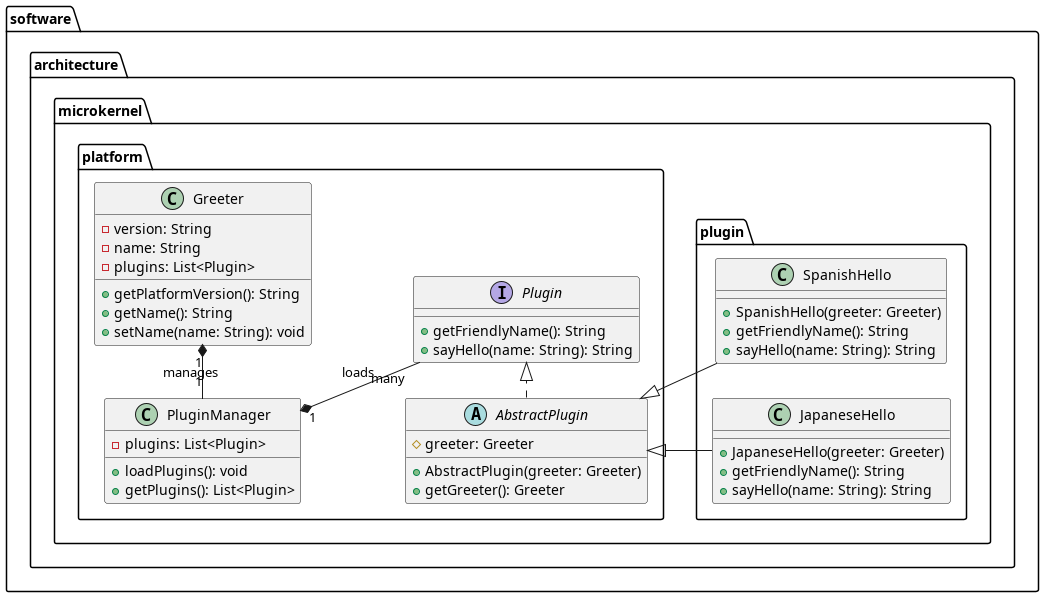
\includegraphics[width=0.9\textwidth]{../../images/out/plugin_architecture}
\label{fig:plugin_architecture}
\end{figure}
\end{frame}

\subsection{Plugin Interface}

\begin{frame}{Plugin Interface Overview}
\vspace{20pt}
\begin{columns}[t]
\column{0.5\textwidth}
\begin{itemize}
	\item \texttt{Plugin} interface acts as a contract for all plugins.
	\item Allows system interaction with various plugin implementations without relying on internal details.
	\item Supports modularity and flexibility in microkernel.
\end{itemize}
\column{0.5\textwidth}
\begin{itemize}
	\item Defines two main methods:
	\begin{itemize}
		\item \texttt{getFriendlyName()} – Returns plugin's friendly name.
		\item \texttt{sayHello(String name)} – Returns customised greeting.
	\end{itemize}
	\item Follows \textbf{Open/Closed Principle (OCP)} to allow easy system extension.
\end{itemize}
\end{columns}
\end{frame}

\begin{frame}[fragile]{Plugin Interface Code}
\vspace{20pt}
\begin{lstlisting}[style=JavaStyle]
package software.architecture.microkernel.platform;

public interface Plugin {
	String getFriendlyName();
	String sayHello(String name);
}
\end{lstlisting}
\end{frame}

\subsection{AbstractPlugin Class}

\begin{frame}{AbstractPlugin Class Overview}
\vspace{20pt}
\begin{columns}[t]
\column{0.5\textwidth}
\begin{itemize}
	\item \texttt{AbstractPlugin} provides base implementation of \texttt{Plugin} interface.
	\item Serves as superclass for all plugins.
	\item Simplifies creation of new plugins by handling common logic.
\end{itemize}
\column{0.5\textwidth}
\begin{itemize}
	\item Key components:
	\begin{itemize}
		\item \texttt{implements Plugin}: Forces method implementation.
		\item \texttt{protected Greeter greeter}: Access to \texttt{Greeter} instance.
		\item Constructor assigns \texttt{Greeter} reference.
	\end{itemize}
	\item Promotes code reuse and system extensibility.
\end{itemize}
\end{columns}
\end{frame}

\begin{frame}[fragile]{AbstractPlugin Class Code}
\vspace{20pt}
\begin{lstlisting}[style=JavaStyle]
package software.architecture.microkernel.platform;

public abstract class AbstractPlugin implements Plugin {
	protected Greeter greeter;
	
	public AbstractPlugin(Greeter greeter) {
		this.greeter = greeter;
	}
}
\end{lstlisting}
\end{frame}

\subsection{SpanishHello Class}

\begin{frame}{SpanishHello Class Overview}
\vspace{20pt}
\begin{columns}[t]
\column{0.5\textwidth}
\begin{itemize}
	\item \texttt{SpanishHello} implements the \texttt{Plugin} interface by extending \texttt{AbstractPlugin}.
	\item Provides greeting in Spanish.
	\item Gains access to \texttt{Greeter} through superclass.
\end{itemize}
\column{0.5\textwidth}
\begin{itemize}
	\item Key elements:
	\begin{itemize}
		\item \texttt{extends AbstractPlugin}: Inherits basic functionality.
		\item Constructor: Receives \texttt{Greeter}, prints load message.
		\item \texttt{getFriendlyName()}: Returns "Greet in Spanish".
		\item \texttt{sayHello(String name)}: Returns greeting \texttt{"Hola, <name>!"}.
	\end{itemize}
\end{itemize}
\end{columns}
\end{frame}

\begin{frame}[fragile]{SpanishHello Class Code}
\vspace{20pt}
\begin{lstlisting}[style=JavaStyle, basicstyle=\tiny\ttfamily]
package software.architecture.microkernel.plugin;

import software.architecture.microkernel.platform.Greeter;
import software.architecture.microkernel.platform.AbstractPlugin;

public class SpanishHello extends AbstractPlugin {
	
	public SpanishHello(Greeter greeter) {
		super(greeter);
		System.out.println(getFriendlyName() + " is loaded by Greeter "
		+ greeter.getPlatformVersion());
	}
	
	@Override
	public String getFriendlyName() {
		return "Greet in Spanish";
	}
	
	@Override
	public String sayHello(String name) {
		return "Hola, " + name + "!";
	}
}
\end{lstlisting}
\end{frame}

\subsection{JapaneseHello Class}

\begin{frame}{JapaneseHello Class Overview}
\vspace{20pt}
\begin{columns}[t]
\column{0.5\textwidth}
\begin{itemize}
	\item \texttt{JapaneseHello} is another plugin implementation extending \texttt{AbstractPlugin}.
	\item Provides greeting in Japanese.
	\item Accesses \texttt{Greeter} through superclass.
\end{itemize}
\column{0.5\textwidth}
\begin{itemize}
	\item Key elements:
	\begin{itemize}
		\item \texttt{extends AbstractPlugin}: Inherits basic structure.
		\item Constructor: Receives \texttt{Greeter}, prints load message.
		\item \texttt{getFriendlyName()}: Returns "Greet in Japanese".
		\item \texttt{sayHello(String name)}: Returns greeting \texttt{"XXXXX, <name>!"}.
	\end{itemize}
\end{itemize}
\end{columns}
\end{frame}

\begin{frame}[fragile]{JapaneseHello Class Code}
\vspace{20pt}
\begin{lstlisting}[style=JavaStyle, inputencoding=utf8, basicstyle=\tiny\ttfamily]
package software.architecture.microkernel.plugin;

import software.architecture.microkernel.platform.Greeter;
import software.architecture.microkernel.platform.AbstractPlugin;

public class JapaneseHello extends AbstractPlugin {
	
	public JapaneseHello(Greeter greeter) {
		super(greeter);
		System.out.println(getFriendlyName() + " is loaded by Greeter "
		+ greeter.getPlatformVersion());
	}
	
	@Override
	public String getFriendlyName() {
		return "Greet in Japanese";
	}
	
	@Override
	public String sayHello(String name) {
		return "こんにちは, " + name + "!";
	}
}
\end{lstlisting}
\end{frame}



\subsection{PluginManager Class}

\begin{frame}[fragile]{PluginManager: Declaration and Constructor}
\vspace{20pt}
\begin{lstlisting}[style=JavaStyle, inputencoding=utf8, basicstyle=\tiny\ttfamily]
package software.architecture.microkernel.platform;

import java.io.File;
import java.io.InputStream;
import java.lang.reflect.Constructor;
import java.net.URL;
import java.net.URLClassLoader;
import java.util.*;

public class PluginManager {
	
	private final Greeter greeter;
	private final List<Plugin> plugins = new ArrayList<>();
	
	public PluginManager(Greeter greeter) {
		this.greeter = greeter;
	}
\end{lstlisting}

\begin{itemize}
	\item Declares the \texttt{PluginManager} class to manage plugin lifecycle.
	\item Holds reference to \texttt{Greeter} and a list to store loaded plugins.
	\item Constructor receives \texttt{Greeter} instance to pass to plugins.
\end{itemize}
\end{frame}

\begin{frame}[fragile]{PluginManager: Begin \texttt{loadPlugins()}}
\vspace{20pt}
\begin{lstlisting}[style=JavaStyle, inputencoding=utf8, basicstyle=\scriptsize\ttfamily]
	public void loadPlugins() {
		try {
			File pluginDir = new File("plugins");
			if (!pluginDir.exists() || !pluginDir.isDirectory()) {
				System.out.println("No plugins directory found.");
				return;
			}
		\end{lstlisting}
		
		\begin{itemize}
			\item Defines \texttt{loadPlugins()} method to dynamically load plugins.
			\item Checks if \texttt{plugins/} directory exists and is valid.
			\item Exits if directory not found.
		\end{itemize}
	\end{frame}
	
	\begin{frame}[fragile]{PluginManager: Locate JAR Files}
		\vspace{20pt}
		\begin{lstlisting}[style=JavaStyle, inputencoding=utf8, basicstyle=\scriptsize\ttfamily]
			File[] jarFiles = pluginDir.listFiles((dir, name) -> name.endsWith(".jar"));
			if (jarFiles == null || jarFiles.length == 0) {
				System.out.println("No plugins found.");
				return;
			}
		\end{lstlisting}
		
		\begin{itemize}
			\item Filters `.jar` files in \texttt{plugins/} directory.
			\item Checks if any plugin files are found.
			\item Exits if no valid `.jar` files.
		\end{itemize}
	\end{frame}
	
	\begin{frame}[fragile]{PluginManager: Load Plugin JARs}
		\vspace{20pt}
		\begin{lstlisting}[style=JavaStyle, inputencoding=utf8, basicstyle=\tiny\ttfamily]
			for (File jar : jarFiles) {
				URLClassLoader classLoader = new URLClassLoader(
				new URL[]{jar.toURI().toURL()},
				getClass().getClassLoader()
				);
				InputStream propertiesInputStream =
				classLoader.getResourceAsStream("plugin.properties");
				
				if (propertiesInputStream == null) {
					System.out.println("Missing plugin.properties in " + jar.getName());
					continue;
				}
			\end{lstlisting}
			
			\begin{itemize}
				\item Iterates over each `.jar` file.
				\item Creates \texttt{URLClassLoader} for each plugin.
				\item Loads \texttt{plugin.properties} file to read plugin configuration.
				\item Skips plugin if properties file not found.
			\end{itemize}
		\end{frame}
		
		\begin{frame}[fragile]{\LARGE{PluginManager: Read Properties}}
			\vspace{20pt}
			\begin{lstlisting}[style=JavaStyle, inputencoding=utf8, basicstyle=\scriptsize\ttfamily]
				Properties properties = new Properties();
				properties.load(propertiesInputStream);
				String mainClassName = properties.getProperty("mainclass");
				
				if (mainClassName == null || mainClassName.isEmpty()) {
					System.out.println("Invalid mainclass entry in " + jar.getName());
					continue;
				}
			\end{lstlisting}
			
			\begin{itemize}
				\item Loads plugin configuration using \texttt{Properties}.
				\item Retrieves \texttt{mainclass} entry for plugin main class.
				\item Skips plugin if \texttt{mainclass} is invalid or empty.
			\end{itemize}
		\end{frame}
		
		\begin{frame}[fragile]{\LARGE{PluginManager: Reflection-Based Initialisation}}
			\vspace{20pt}
			\begin{lstlisting}[style=JavaStyle, inputencoding=utf8, basicstyle=\scriptsize\ttfamily]
				Class<?> classToLoad = Class.forName(
				mainClassName, true, classLoader
				);
				Class<? extends Plugin> pluginClass =
				classToLoad.asSubclass(Plugin.class);
				Constructor<? extends Plugin> constructor =
				pluginClass.getDeclaredConstructor(Greeter.class);
				Plugin plugin = constructor.newInstance(greeter);
				plugins.add(plugin);
			\end{lstlisting}
			
			\begin{itemize}
				\item Dynamically loads plugin class using \texttt{Class.forName()}.
				\item Verifies the class implements \texttt{Plugin}.
				\item Uses reflection to call constructor with \texttt{Greeter} argument.
				\item Adds loaded plugin to \texttt{plugins} list.
			\end{itemize}
		\end{frame}
		
		\begin{frame}[fragile]{\LARGE{PluginManager: Exception Handling and Accessor}}
			\vspace{20pt}
			\begin{lstlisting}[style=JavaStyle, inputencoding=utf8, basicstyle=\scriptsize\ttfamily]
			}
		} catch (Exception e) {
			e.printStackTrace();
		}
	}
	
	public List<Plugin> getPlugins() {
		return plugins;
	}
}
\end{lstlisting}

\begin{itemize}
\item Surrounds loading logic with exception handling.
\item Logs errors if any part of plugin loading fails.
\item Provides \texttt{getPlugins()} method to access loaded plugins.
\end{itemize}
\end{frame}


\subsection{Greeter Class}

\begin{frame}[fragile]{Greeter: Declaration and Attributes}
	\vspace{20pt}
	\begin{lstlisting}[style=JavaStyle, inputencoding=utf8, basicstyle=\scriptsize\ttfamily]
		package software.architecture.microkernel.platform;
		
		import java.io.BufferedReader;
		import java.io.InputStreamReader;
		import java.util.List;
		
		public class Greeter {
			
			private final String version = "v1.0.1";
			private String name = "Alice";
			private final PluginManager pluginManager;
		\end{lstlisting}
		
		\begin{itemize}
			\item Declares \texttt{Greeter} as the core of Microkernel platform.
			\item Holds platform version, user name, and \texttt{PluginManager}.
			\item Manages plugin loading and user interaction.
		\end{itemize}
	\end{frame}
	
	\begin{frame}[fragile]{\LARGE{Greeter: Constructor and PluginManager Initialisation}}
		\vspace{20pt}
		\begin{lstlisting}[style=JavaStyle, inputencoding=utf8, basicstyle=\scriptsize\ttfamily]
			public Greeter() {
				this.pluginManager = new PluginManager(this);
				this.pluginManager.loadPlugins();
			}
		\end{lstlisting}
		
		\begin{itemize}
			\item Constructor initialises \texttt{PluginManager}.
			\item Immediately loads available plugins.
			\item Integrates plugins dynamically at runtime.
		\end{itemize}
	\end{frame}
	
	\begin{frame}[fragile]{Greeter: Main Method}
		\vspace{20pt}
		\begin{lstlisting}[style=JavaStyle, inputencoding=utf8, basicstyle=\scriptsize\ttfamily]
			public static void main(String[] args) {
				Greeter greeter = new Greeter();
				greeter.run();
			}
		\end{lstlisting}
		
		\begin{itemize}
			\item Entry point of the application.
			\item Creates an instance of \texttt{Greeter}.
			\item Calls \texttt{run()} method to start interactive session.
		\end{itemize}
	\end{frame}
	
	\begin{frame}[fragile]{Greeter: User Interface Loop (Part 1)}
		\vspace{20pt}
		\begin{lstlisting}[style=JavaStyle, inputencoding=utf8, basicstyle=\scriptsize\ttfamily]
			public void run() {
				try (BufferedReader reader = new BufferedReader(
				new InputStreamReader(System.in))) {
					while (true) {
						System.out.println("Select the language to greet in:");
						List<Plugin> plugins = pluginManager.getPlugins();
						for (int i = 0; i < plugins.size(); i++) {
							System.out.println((i + 1) + ". " + 
							plugins.get(i).getFriendlyName());
						}
						System.out.println("0. Quit");
						System.out.print("Input: ");
					\end{lstlisting}
					
					\begin{itemize}
						\item \texttt{run()} method presents a CLI menu.
						\item Lists all loaded plugins with friendly names.
						\item Prompts user for plugin selection input.
					\end{itemize}
				\end{frame}
				
				\begin{frame}[fragile]{Greeter: User Interface Loop (Part 2)}
					\vspace{20pt}
					\begin{lstlisting}[style=JavaStyle, inputencoding=utf8, basicstyle=\scriptsize\ttfamily]
						int menu = Integer.parseInt(reader.readLine()) - 1;
						if (menu == -1) break;
						
						if (menu >= 0 && menu < plugins.size()) {
							System.out.println("\n" + 
							plugins.get(menu).sayHello(name) + "\n");
						} else {
							System.out.println("Invalid selection. Try again.");
						}
					}
					System.out.println("Quit. Thanks for playing!");
				} catch (Exception e) {
					e.printStackTrace();
				}
			}
		\end{lstlisting}
		
		\begin{itemize}
			\item Handles user input and plugin selection, executes selected plugin's \texttt{sayHello()} method, and allows clean exit on input \texttt{0}.
		\end{itemize}
	\end{frame}
	
	\begin{frame}[fragile]{Greeter: Accessor Methods}
		\vspace{20pt}
		\begin{lstlisting}[style=JavaStyle, inputencoding=utf8, basicstyle=\scriptsize\ttfamily]
			public String getPlatformVersion() {
				return version;
			}
			
			public String getName() {
				return name;
			}
		}
	\end{lstlisting}
	
	\begin{itemize}
		\item Provides methods for plugins to access platform version and user name.
		\item Enables plugins to personalise greetings and display platform details.
	\end{itemize}
\end{frame}

\section{Compilation and Running the Application}

\begin{frame}[fragile]{Compilation and Running Overview}
	\vspace{20pt}
	\begin{itemize}
		\item Microkernel-based application uses \textbf{Maven} for build and dependency management.
		\item Process consists of:
		\begin{enumerate}
			\item Building the main platform project (\texttt{Greeter}).
			\item Building each plugin as a separate Maven project.
			\item Moving compiled \texttt{.jar} plugin files to \texttt{plugins/} folder.
			\item Running the platform application, auto-loading available plugins.
		\end{enumerate}
	\end{itemize}
\end{frame}

\subsection{Building and Installing Platform Project}

\begin{frame}[fragile]{Building Platform and Plugins}
	\vspace{20pt}
	\begin{columns}[t]
		\column{0.5\textwidth}
		\textbf{Building Platform Project}
		
		To build the main platform project containing \texttt{Greeter}, run:
		
		\begin{lstlisting}[language=bash, basicstyle=\footnotesize\ttfamily]
			mvn clean package install
		\end{lstlisting}
		
		\textbf{Maven Tasks:}
		\begin{itemize}
			\item Downloads and manages required dependencies.
			\item Compiles platform source code.
			\item Generates \texttt{.jar} in \texttt{target/} directory.
		\end{itemize}
		
		\column{0.5\textwidth}
		\textbf{Building Plugins}
		
		Each plugin, such as \texttt{JapaneseHello} or \texttt{SpanishHello}, is built separately. Navigate to each plugin directory and run:
		
		\begin{lstlisting}[language=bash, basicstyle=\footnotesize\ttfamily]
			mvn clean package
		\end{lstlisting}
		
		\begin{itemize}
			\item Output placed in \texttt{target/}.
			\item Plugin \texttt{.jar} name based on \texttt{pom.xml}.
		\end{itemize}
	\end{columns}
\end{frame}

\begin{frame}[fragile]{Moving Plugins and Running Platform}
	\vspace{20pt}
	\begin{columns}[t]
		\column{0.5\textwidth}
		\textbf{Moving Plugin JARs}
		
		Move compiled plugin \texttt{.jar} files to platform’s plugin directory:
		
		\begin{lstlisting}[language=bash, basicstyle=\footnotesize\ttfamily]
			mv target/*.jar ../platform/plugins/
		\end{lstlisting}
		
		\begin{itemize}
			\item Ensures platform detects plugins at runtime.
			\item Simplifies plugin deployment.
		\end{itemize}
		
		\column{0.5\textwidth}
		\textbf{Running the Platform Application}
		
		Run the \texttt{Greeter} app:
		
		\begin{lstlisting}[language=bash, basicstyle=\footnotesize\ttfamily]
			mvn run 
			# or
			java -jar target/platform.jar
		\end{lstlisting}
		
		\begin{itemize}
			\item Plugins auto-loaded from \texttt{plugins/}.
			\item Greeting options displayed dynamically.
		\end{itemize}
	\end{columns}
\end{frame}


\subsection{Sample Program Output}

\begin{frame}[fragile]{Program Output Example}
	\vspace{20pt}
	\begin{lstlisting}[language=bash, basicstyle=\tiny\ttfamily]
		Greet in Japanese is loaded by Greeter v1.0.1
		Greet in Spanish is loaded by Greeter v1.0.1
		Select the language to greet in:
		1. Greet in Japanese
		2. Greet in Spanish
		0. Quit
		Input: 1
		
		こんにちは, Alice!
		
		Select the language to greet in:
		1. Greet in Japanese
		2. Greet in Spanish
		0. Quit
		Input: 2
		
		Hola, Alice!
		
		Select the language to greet in:
		1. Greet in Japanese
		2. Greet in Spanish
		0. Quit
		Input:
	\end{lstlisting}
\end{frame}

\begin{frame}[fragile]{Summary of the Project}
	\vspace{20pt}
	\begin{itemize}
		\item Plugins are compiled and packaged separately.
		\item No need to modify or recompile core source code to extend functionality.
		\item Simply add compiled plugin \texttt{.jar} to \texttt{plugins/} directory.
		\item Promotes a flexible, modular architecture.
	\end{itemize}
\end{frame}

\section{Conclusion}

\begin{frame}{Conclusion}
	\vspace{15pt}
	\begin{itemize}
		\item \textbf{Microkernel} and \textbf{plugin} architectures improve modularity, flexibility, \& scalability
		
		\item \textbf{Plugin Architecture:}
		\begin{itemize}
			\item Adds features dynamically without altering core code.
			\item Common in IDEs, CMS, game engines.
			\item Supports scalability and easier maintenance.
		\end{itemize}
		
		\item \textbf{Java Implementation:} Demonstrates plugin loading via reflection, dependency handled by Maven.
		
		\item Developers can choose suitable architecture based on system needs for flexibility and reliability.
	\end{itemize}
\end{frame}


\end{document}
